\section{Numerical Experiments}

\subsection{Travelling Wave Allen Cahn}
In this section, we run numerical experiments comparing the backward Euler method to Krylov methods for computing solutions to a PDE.
Specifically, we will investigate the initial boundary value problem for the Allen Cahn equation on a strip with a travelling wave solution\cite{YukitakaFukao2004} given by:

\begin{align*}
    \hat u(x,y,t)&=\frac{e^{\frac{x-ct}{\sqrt2}}}{1+e^{\frac{x-ct}{\sqrt2}}} \label{TravellingWaveSol}\\
    \text{where } c &= \frac{\sqrt{2}}{4}
\end{align*}
and where the problem is defined as follows:
\begin{align*}
    u_t&=\Delta u+u(u-\frac14)(1-u) \text{ $(x,y,t)\in \mathbb{R} \times (-1,1) \times [0, 8]$}\\
    u_0(x, y) &= \hat u(x,y, 0)
\end{align*}
With homogeneous Neumann boundary conditions along the top and bottom of the domain.

However, for our numerical experiments we compute on the space $\Omega=(-16,16)\times(-1,1)$ and enforce the following Neumann boundary conditions along the left and right boundaries.
\begin{align*}
    \nabla u \cdot \hat n &= g \text{ for $g = \nabla \hat u \cdot \hat n$}
\end{align*}
Where $\hat n$ is the unit normal on the boundary.

Where $u$ is the solution, we write it in weak form:
\begin{align*}
    \dot u&=\Delta u+u(u-\frac14)(1-u)\\
    \int_{\Omega} \dot u v &=\int_{\Omega} \Delta uv+u(u-\frac14)(1-u)v \text{ for a smooth function $v \in C^{\infty}(\overline{\Omega})$}\\
    \int_{\Omega} \dot u v &=\int_{\Omega} u(u-\frac14)(1-u)v - \nabla u \cdot \nabla v + \int_{\partial\Omega}  v\hat n \cdot \nabla \hat u\\
\end{align*}
We now introduce our finite element space $V_h$ for a spacial discretization size of $h \in \mathbb{R}$.
We can now substitute in $u_h(t,x,y) = \sum_i u_i(t) v_i(x,y)$ where $u_i \in \mathbb{R}$ and $v_i \in V_h$ for $i,j = 0,1,...,dim(V_h)$.
\begin{align*}
    \text{we get } \sum_i\int_{\Omega} \dot u_i v_i v_j &=\sum_i(\int_{\Omega} u_iv_i(u_iv_i-\frac14)(1-u_iv_i)v_j - \int_{\Omega}\nabla (u_iv_i) \cdot \nabla v_j + \int_{\partial\Omega}  v_j\hat n \cdot \nabla \hat u_iv_i)\\
    \sum_iu_i\int_{\Omega}v_iv_j &= -u_i\sum_i(\int_{\Omega}\nabla v_i \cdot \nabla v_j + \int_{\Omega}R(u_h)v_j)\\
    \text{where we have } R(u)&=u(u-\frac14)(1-u) + \int_{\partial\Omega}  \hat n \cdot \nabla \hat  u\\
    \intertext{The above is true for all $i,j$. Writing in matrix vector form gives}
    M \underline{\dot u} &= DN(\underline{u})\underline{u} + R(\underline{u})\\
    \text{where } M_{i,j} &= \int_{\Omega}v_iv_jdx
\end{align*}
In the tests, we will investigate the relationship between step size, $L_2$ error given by $||\hat u - u_h||_{L_2}$ and calls to the operator $N$ which will be a crude approximation to the computational cost.
We compare the backward Euler, first and second order exponential methods over grid sizes: $128 \times 8$ and $256 \times 8$ and with time step $\tau=8,4,2,1,0.5,0.25,0.125,0.0625,0.03125$.

\subsubsection{Experimental Results}

Below, we show the $L_2$ error with respect to the time step $\tau$.
Where in the legend EXP1LAN 16 denotes the first order method with equipped with the Lanzcos algorithm, Krylov size 16, likewise for EXP2LAN and the second order method.
BE denotes the backwards Euler method.

\begin{figure}[H]
    \centering
    \begin{minipage}{0.49\textwidth}
        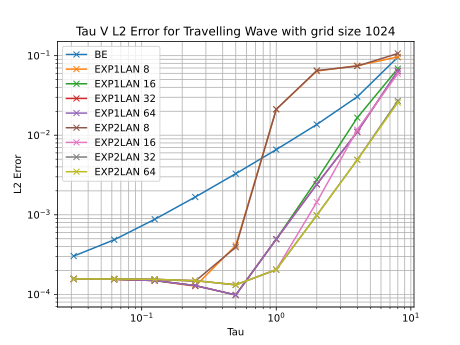
\includegraphics[width=1\textwidth]{Graphs/TravellingWave/Tau V L2 Error for Travelling Wave with grid size 1024.png} % Change filename to your image
        \caption{$\tau$ vs $L_2$ with grid size 1024}
        \label{fig:plot1}
    \end{minipage}\hfill
    \centering
    \begin{minipage}{0.49\textwidth}
        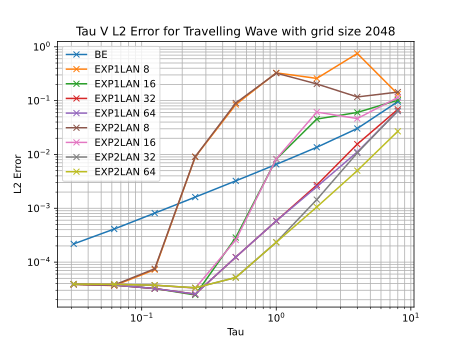
\includegraphics[width=1\textwidth]{Graphs/TravellingWave/Tau V L2 Error for Travelling Wave with grid size 2048.png} % Change filename to your image
        \caption{$\tau$ vs $L_2$ with grid size 2048}
        \label{fig:plot2}
    \end{minipage}\hfill
\end{figure}

Firstly, note that all of the methods tested converge, tending towards an apparent minimum error, with the exponential methods levelling out.
This minimum error is lower for a finer spacial discretization suggesting that the minimum error is the result of the spacial discretization.
The Krylov methods converge faster than the backwards Euler method for a Krylov size equal to or larger than 32 as shown by the steeper graph.
The performance of the first and second order methods seem simillar both in terms of error and rate of convergence.
We notice that when a smaller Krylov subspace, is used the exponential methods only start to converge for a sufficiently small $\tau$.
Likewise, when these methods start to converge, we observe that they perform similarly to the methods using a larger subspace.
However, they will require fewer operator calls.
This suggests that, for sufficiently small timesteps, a shallower subspace may suffice.
In contrast, larger timesteps require a deeper Krylov subspace.
As a result, it is important to look into whether it is more efficient to have a smaller Krylov subspace and $\tau$ or a larger space with corresponding larger $\tau$.

Next we will look into operator calls in order to quantify this difference in performance.
We compare the error with the number of calls to the operator.
These operator calls are needed for computing $N$ which is used with the matrix free methods as described above as well as for computing the non-linear term $R$.

\begin{figure}[H]
    \centering
    \begin{minipage}{0.49\textwidth}
        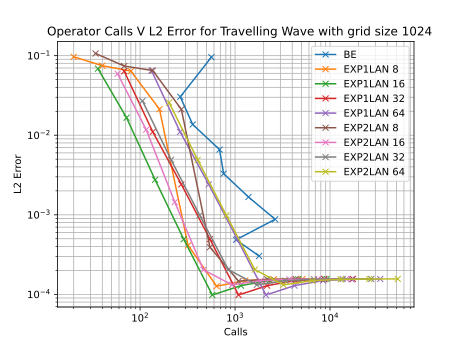
\includegraphics[width=1\textwidth]{Graphs/TravellingWave/Operator Calls V Error for Travelling Wave with grid size 1024.png} % Change filename to your image
        \caption{Operator calls vs $L_2$ with grid size 1024}
        \label{fig:plot1}
    \end{minipage}\hfill
    \centering
    \begin{minipage}{0.49\textwidth}
        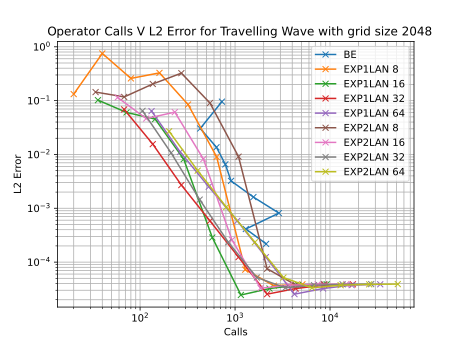
\includegraphics[width=1\textwidth]{Graphs/TravellingWave/Operator Calls V Error for Travelling Wave with grid size 2048.png} % Change filename to your image
        \caption{Operator calls vs $L_2$ with grid size 2048}
        \label{fig:plot2}
    \end{minipage}\hfill
\end{figure}

As expected, when a larger Krylov subspace is used, more calls to the operator are required.
This can be seen by comapring the first order exponential integrator with Krylov sizes 16 and 32, where both are identical but the latter has been shifted to the right, using double the number of operator calls.
The backward Euler method appears somewhat erratic.
This is due to the use of an internal Newton solver which does not have a fixed requirement for number of calls to the operator, instead, running until a given tolerance is reached.
We also observe that the exponential methods outperform the BE by achieving a lower error with fewer calls to the operator.
We also see that before the discretization error is reached, a Krylov size of 16 gives the lowest error for a given number of operator calls.

Here we present the experimental orders of convergence for the grid size 1024.

\begin{table}[H]
    \centering
    \begin{tabular}{| c | c | c | c |}
    \hline
    $\tau$ & BE & EXP1LAN 64 & EXP2LAN 64 \\
    \hline
    4 & 1.6562 & 2.5200 & 2.4275 \\
    2 & 1.1560 & 2.1472 & 2.2449 \\
    1 & 1.0544 & 2.1084 & 2.1753 \\
    0.5 & 1.0189 & 2.2355 & 2.1762 \\
    0.25 & 1.0017 & 2.2848 & 0.6355 \\
    0.125 & 0.9875 & -0.3464 & -0.1611 \\
    0.0625 & 0.9808 & -0.2097 & -0.0546 \\
    0.03125 & 0.9193 & -0.0516 & -0.0141 \\
    \hline
    \end{tabular}
    \caption{Experimental orders of convergence}
    \label{tab:EOCs}
\end{table}


We observe that the rate of convergence for the second order method was in line with what has been shown analytically\cite{Huang2022}, converging at a rate of $2$.
The first order method converges with a rate of 2 despite an expectation of a rate of $1$\cite{Huang2022}.
The exponential methods stop converging as they reach the discretization error.
The backwards Euler converges at the rate expected of 1.

\subsection{A 2D Allen Cahn Problem}
The above problem, while done on a two dimensional domain, is really a one dimensional problem.
We wish to see how these results carry over to a truly two dimensional problem. 
We will now begin looking into a two dimensional Allen Cahn Problem given by:
\begin{align*}
    u_t &= -\Delta u + u (u^2-1) \text{ } \Omega=[0,1]\times[0,1], 0\leq t \leq T
\end{align*}
with Neumann boundary conditions.
The initial condition is chosen by randomly setting points on the grid from a uniform distribution in the range $-0.9,0.9$.
The same randomly generated initial condition will be used for each test.
As we do not have an exact solution, we will use the backwards Euler method with a timestep of $\tau = 10^{-4}$ to genarate a reference solution.
We will compare the backwards Euler method to the first and second order exponential integrator methods described above.
The tests are run on a $60\times60$ grid with the end time being $T=24$.
The error is computed by calculating the $L_2$ error between the prediction of the chosen stepper and the reference solution. 
Below we present our results.

\subsubsection{Experimental Results}

We begin by comparing the timestep size $\tau$ to the $L_2$ error for the different methods.

\begin{figure}[H]
    \centering
    \begin{minipage}{0.49\textwidth}
        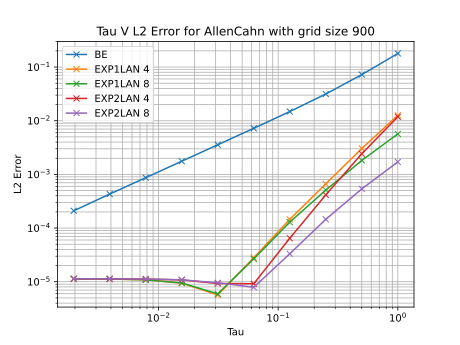
\includegraphics[width=1\textwidth]{Graphs/AllenCahn/Tau V L2 Error for AllenCahn with grid size 900.png} % Change filename to your image
        \caption{$\tau$ vs $L_2$ with grid size 900}
        \label{fig:ACtauE}
    \end{minipage}\hfill
    \centering
    \begin{minipage}{0.49\textwidth}
        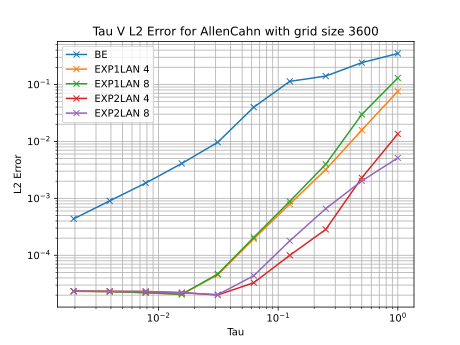
\includegraphics[width=1\textwidth]{Graphs/AllenCahn/Tau V L2 Error for AllenCahn with grid size 3600.png} % Change filename to your image
        \caption{$\tau$ vs $L_2$ with grid size 3600}
        \label{fig:ACtauE1024}
    \end{minipage}\hfill
\end{figure}

We observe convergence in error for both expoential methods for both Krylov sizes.
These methods significantly outperform the backwards Euler method, similar to the travelling wave Allen Cahn problem given above.
They reach the discretization error at around $\tau=3\times10^{-2}$ significantly ahead of the backwards Euler method, which will need a timestep size more than ten times smaller to achieve the same error.
For this problem, a relatively shallow subspace has been used compared to above and appears to be sufficient.

Again, we present the number of calls to the operator against the error:
\begin{figure}[H]
    \centering
    \begin{minipage}{0.49\textwidth}
        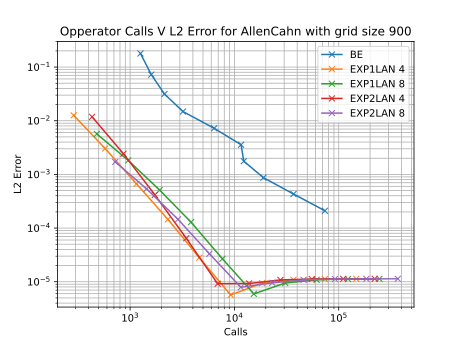
\includegraphics[width=1\textwidth]{Graphs/AllenCahn/Operator Calls V Error for AllenCahn with grid size 900.png} % Change filename to your image
        \caption{Operator calls vs $L_2$ with grid size 900}
        \label{fig:plot1}
    \end{minipage}\hfill
    \centering
    \begin{minipage}{0.49\textwidth}
        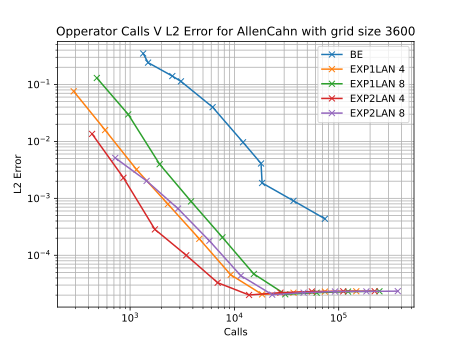
\includegraphics[width=1\textwidth]{Graphs/AllenCahn/Operator Calls V Error for AllenCahn with grid size 3600.png} % Change filename to your image
        \caption{Operator calls vs $L_2$ with grid size 3600}
        \label{fig:plot2}
    \end{minipage}\hfill
\end{figure}
For all methods, we see that to achieve a lower error requires more calls to the operator.
We see that in terms of performance the backwards Euler method performs significantly worse in comparison to both of the exponential methods.
The exponential methods reach convergence at around $10^4$ operator calls.

Here we present the experimental orders of convergence on a grid size of 3600.

\begin{table}[H]
    \centering
    \begin{tabular}{| c | c | c | c |}
    \hline
    $\tau$ & BE & EXP1LAN 8 & EXP2LAN 8 \\
    \hline
    0.5 & 0.5337 & 2.1244    & 1.3417 \\
    0.25 & 0.7836 & 2.9057    & 1.6172 \\
    0.125 & 0.3088 & 2.1667   & 1.8766 \\
    0.0625 & 1.5046  & 2.0995   & 2.0343 \\
    0.03125 & 2.0486 & 2.1358     & 1.1062 \\
    0.015625 & 1.2371  & 1.1844    & -0.1166 \\
    0.0078125 & 1.1377 & -0.0937 & -0.0679 \\
    0.00390625 & 1.0396 & -0.0652 & -0.0057 \\
    0.001953125 & 1.0482 & -0.0180 & -0.0144 \\
    \hline
    \end{tabular}
    \caption{Experimental orders of convergence}
    \label{tab:reduced_data}
\end{table}

Again, we observe first order convergence for the backwards Euler method with a convergence rate tending towards somewhere between 1 and 1.3.
The exponential methods have a convergence rate in the range of 1.5 to 2.2 showing second order convergence.

\subsection{Reaction Diffusion}

For both of the above problems, the first order exponential method converged with rate 2.
However, we expect the first order exponential method to converge at rate 1.
We wish to measure the performance of this method in comparison to backwards Euler for a problem where it does not converge at rate 2 but at rate 1 as expected.
In order to do this, we study the following reaction diffusion problem\cite{Huang2022}.

\begin{align*}
    u_t &= -\frac12\Delta u + \frac12 \pi^2u + \frac12 \pi^2 e^{-\pi^2t}sin(\pi x)sin(\pi y) \text{ } (x,y)\in\Omega t\in\times[0,t_e]\\
    u(0,x,y) &= (sin(\pi x) - 1)sin(\pi y) \text{ } (x,y)\in \Omega
\end{align*}

With the following exact solution:
\begin{align*}
    u(t, x, y) &= e^{-\pi^2t}(sin(\pi x) - 1)sin(\pi y)
\end{align*}

with homogeneous Dirichlet boundary conditions and where $\Omega = (\frac12, \frac52)\times(0,1)$ and our end time is given by $t_e = 0.1$.
We run our tests on grid sizes of $128\times64$ and $256\times128$ and use times steps sizes of $\tau=\frac{0.1}{2^i}$ for $i = 0,1,...,4$.


We begin by comparing the timestep size $\tau$ to the $L_2$ error for the different methods.
\begin{figure}[H]
    \centering
    \begin{minipage}{0.49\textwidth}
        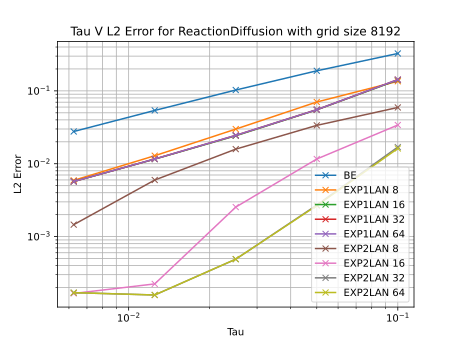
\includegraphics[width=1\textwidth]{Graphs/ReactionDiffusion/Tau V L2 Error for ReactionDiffusion with grid size 8192.png} % Change filename to your image
        \caption{$\tau$ vs $L_2$ with grid size 8192}
        \label{fig:ACtauE}
    \end{minipage}\hfill
    \centering
    \begin{minipage}{0.49\textwidth}
        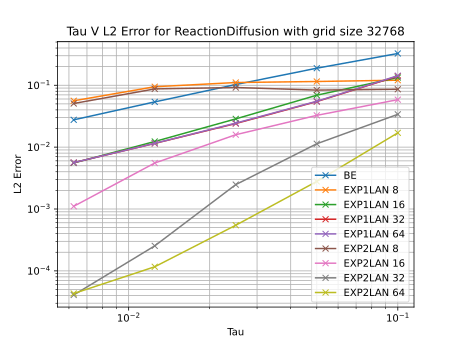
\includegraphics[width=1\textwidth]{Graphs/ReactionDiffusion/Tau V L2 Error for ReactionDiffusion with grid size 32768.png} % Change filename to your image
        \caption{$\tau$ vs $L_2$ with grid size 32768}
        \label{fig:ACtauE1024}
    \end{minipage}\hfill
\end{figure}
All methods appear to converge to the spacial discretization error.
As above, we observe that the Krylov subspace must be sufficiently deep in order to be accurate.
In this example, we can see that the second order method converges at a faster rate than the first order method as the slope for the second order method is steeper.
We also see that the backwards Euler method has a higher error for a given value of $\tau$ the both exponential methods, normally around twice that of the first order expoential integrator method.

Again, we present the number of calls to the operator against the error.
\begin{figure}[H]
    \centering
    \begin{minipage}{0.49\textwidth}
        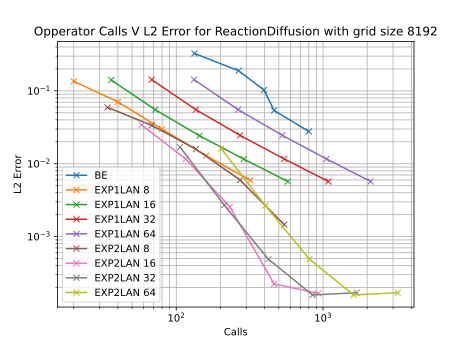
\includegraphics[width=1\textwidth]{Graphs/ReactionDiffusion/Operator Calls V Error for ReactionDiffusion with grid size 8192.png} % Change filename to your image
        \caption{Operator calls vs $L_2$ with grid size 8192}
        \label{fig:plot1}
    \end{minipage}\hfill
    \centering
    \begin{minipage}{0.49\textwidth}
        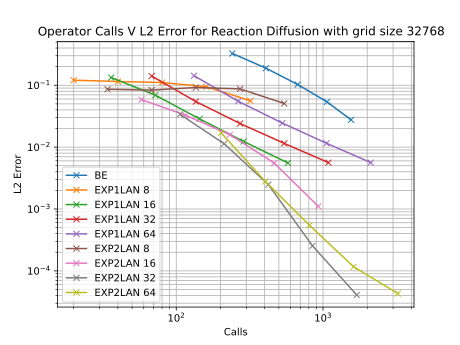
\includegraphics[width=1\textwidth]{Graphs/ReactionDiffusion/Operator Calls V Error for ReactionDiffusion with grid size 32768.png} % Change filename to your image
        \caption{Operator calls vs $L_2$ with grid size 32768}
        \label{fig:plot2}
    \end{minipage}\hfill
\end{figure}
Here we see that for all methods, more operator calls are required to produce results with a smaller error.
The exponential methods achieved a given error with fewer operator calls than the backwards Euler method.
The second order methods required fewer operator calls for a given error than the first order method, especially as the number of calls increased.


Here we present the experimental orders of convergence.
\begin{table}[H]
    \centering
    \begin{tabular}{| c | c | c | c |}
    \hline
    $\tau$ & BE & EXP1LAN 64 & EXP2LAN 64 \\
    \hline
    0.5 & 0.7902 & 1.3717 & 2.6086 \\
    0.25 & 0.8767 & 1.1735 & 2.3519 \\
    0.125 & 0.9320 & 1.0828 & 2.2299\\
    0.0625 & 0.9635  & 1.0378 & 1.4358 \\
    \hline
    \end{tabular}
    \caption{Experimental orders of convergence}
    \label{tab:reduced_data}
\end{table}

Now we observe the expected results, with the first order exponential method converging at rate $1$ and the second order method converging at rate $2$.